\documentclass[border=10pt]{standalone}
\usepackage[svgnames]{xcolor}
\usepackage{amsmath}
\usepackage{pgfplots}
\pgfplotsset{compat=newest}
\usepackage[sfdefault]{FiraSans}
\usepackage{FiraMono}
\renewcommand*\familydefault{\sfdefault}
\begin{document}
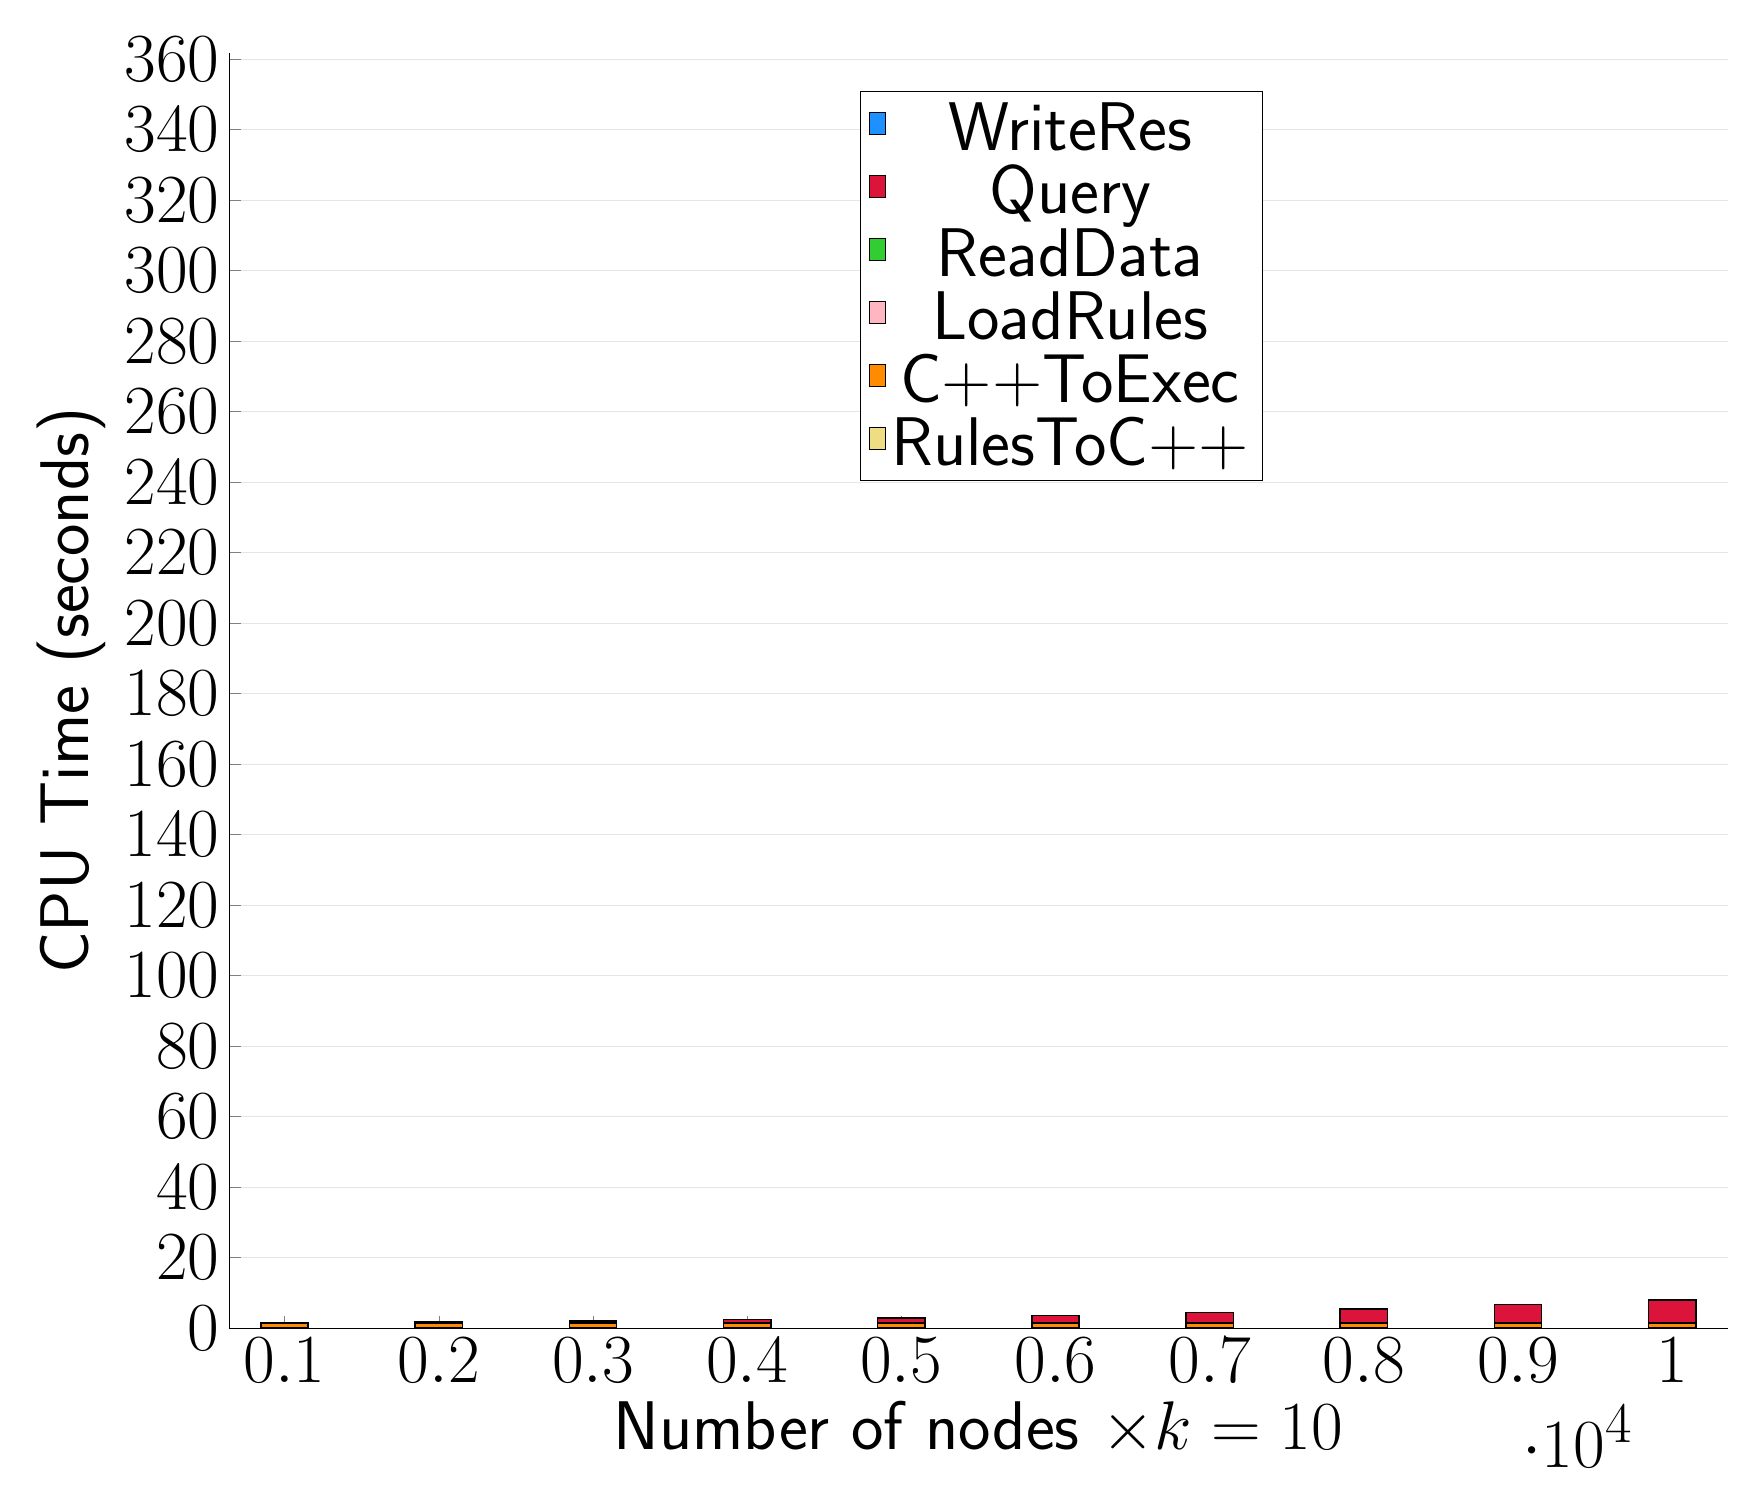
\begin{tikzpicture}
\begin{axis}[
   ybar stacked,
   width=1.7\textwidth,
   bar width=0.6cm,
   ymajorgrids, tick align=inside,
   major grid style={draw=gray!20},
   xtick=data,
   ymin=0, ymax=361.7732,
   axis x line*=bottom,
   axis y line*=left,
   enlarge x limits=0.04,
   legend style={
       at={(0.69, 0.97)},
       anchor=north east,
       legend columns=1,
       font=\Huge,
   },
   ylabel={CPU Time (seconds)},
   xlabel={Number of nodes $\times k=10$},
   label style={font=\Huge},
   tick label style={font=\Huge},
]
\addlegendimage{fill=DodgerBlue, draw=black, line width=0.2pt}
\addlegendentry{WriteRes}
\addlegendimage{fill=Crimson, draw=black, line width=0.2pt}
\addlegendentry{Query}
\addlegendimage{fill=LimeGreen, draw=black, line width=0.2pt}
\addlegendentry{ReadData}
\addlegendimage{fill=LightPink, draw=black, line width=0.2pt}
\addlegendentry{LoadRules}
\addlegendimage{fill=DarkOrange, draw=black, line width=0.2pt}
\addlegendentry{C++ToExec}
\addlegendimage{fill=LightGoldenrod, draw=black, line width=0.2pt}
\addlegendentry{RulesToC++}
\addplot +[fill=LightGoldenrod, draw=black, line width=0.55pt] coordinates {
(1000, 0.006000000000000001)
(2000, 0.004000000000000001)
(3000, 0.004000000000000001)
(4000, 0.008000000000000002)
(5000, 0.004000000000000001)
(6000, 0.006000000000000001)
(7000, 0.010000000000000002)
(8000, 0.010000000000000002)
(9000, 0.008000000000000002)
(10000, 0.006000000000000001)
};
\addplot +[fill=DarkOrange, draw=black, line width=0.55pt] coordinates {
(1000, 1.5059999999999998)
(2000, 1.518)
(3000, 1.5319999999999998)
(4000, 1.528)
(5000, 1.522)
(6000, 1.504)
(7000, 1.518)
(8000, 1.526)
(9000, 1.5059999999999998)
(10000, 1.5180000000000002)
};
\addplot +[fill=LightPink, draw=black, line width=0.55pt] coordinates {
(1000, 0.0001462)
(2000, 0.0001492)
(3000, 0.000147)
(4000, 0.0001508)
(5000, 0.0001472)
(6000, 0.000131)
(7000, 0.00014560000000000002)
(8000, 0.0001442)
(9000, 0.0001508)
(10000, 0.00014600000000000003)
};
\addplot +[fill=LimeGreen, draw=black, line width=0.55pt] coordinates {
(1000, 0.0044858)
(2000, 0.0077492)
(3000, 0.010175)
(4000, 0.012840800000000003)
(5000, 0.015143599999999998)
(6000, 0.016504799999999997)
(7000, 0.0219344)
(8000, 0.0224612)
(9000, 0.025569)
(10000, 0.0277746)
};
\addplot +[fill=Crimson, draw=black, line width=0.55pt] coordinates {
(1000, 0.055281000000000004)
(2000, 0.1879796)
(3000, 0.4528142)
(4000, 0.8673504000000001)
(5000, 1.410262)
(6000, 2.1024320000000003)
(7000, 2.9594180000000003)
(8000, 3.9507419999999995)
(9000, 5.199762000000001)
(10000, 6.522603999999999)
};
\addplot +[fill=DodgerBlue, draw=black, line width=0.55pt] coordinates {
(1000, 0.00020900000000000004)
(2000, 0.000255)
(3000, 0.0002792)
(4000, 0.00035259999999999995)
(5000, 0.0003726)
(6000, 0.00041200000000000004)
(7000, 0.0004378)
(8000, 0.00038359999999999995)
(9000, 0.000374)
(10000, 0.000374)
};
\end{axis}
\end{tikzpicture}

\end{document}
